\section{Learning}

\begin{frame}
	\frametitle{\insertsection}
	\framesubtitle{Learning curve}
	\begin{figure}
		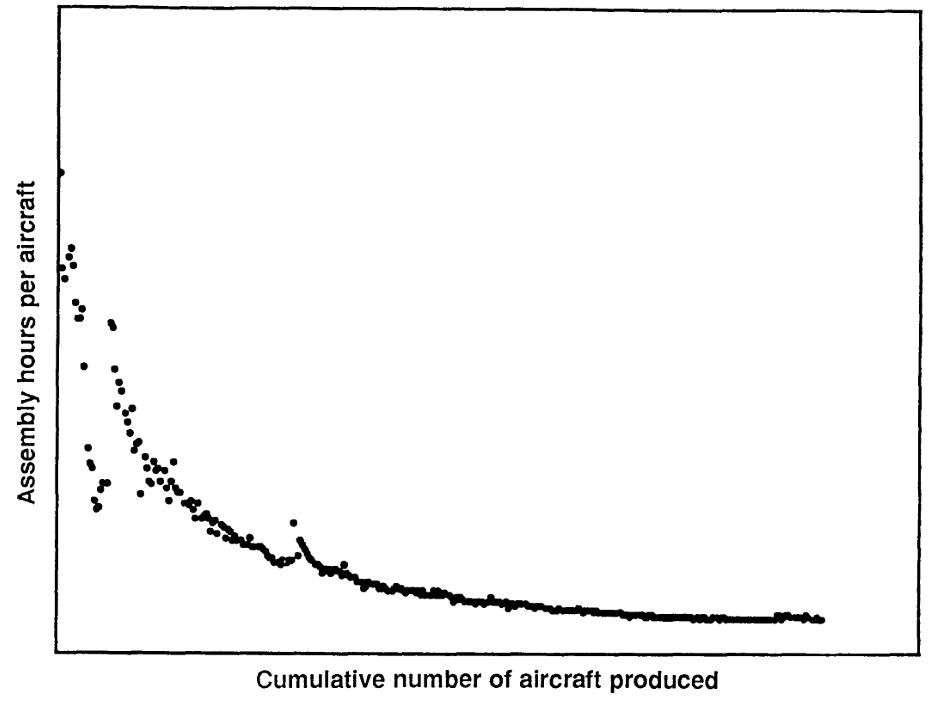
\includegraphics[height=5cm]{resources/learning_curve1.png}
		\caption{Relation between assembly hours per aircraft and cumulative number produced. Units omitted. From: \citet[p. 921]{Argote1990}}
		\note{You have probably seen this before.}
	\end{figure}
\end{frame}

\begin{frame}
	\frametitle{\insertsection}
	\framesubtitle{Disrupted learning}
	\begin{figure}
		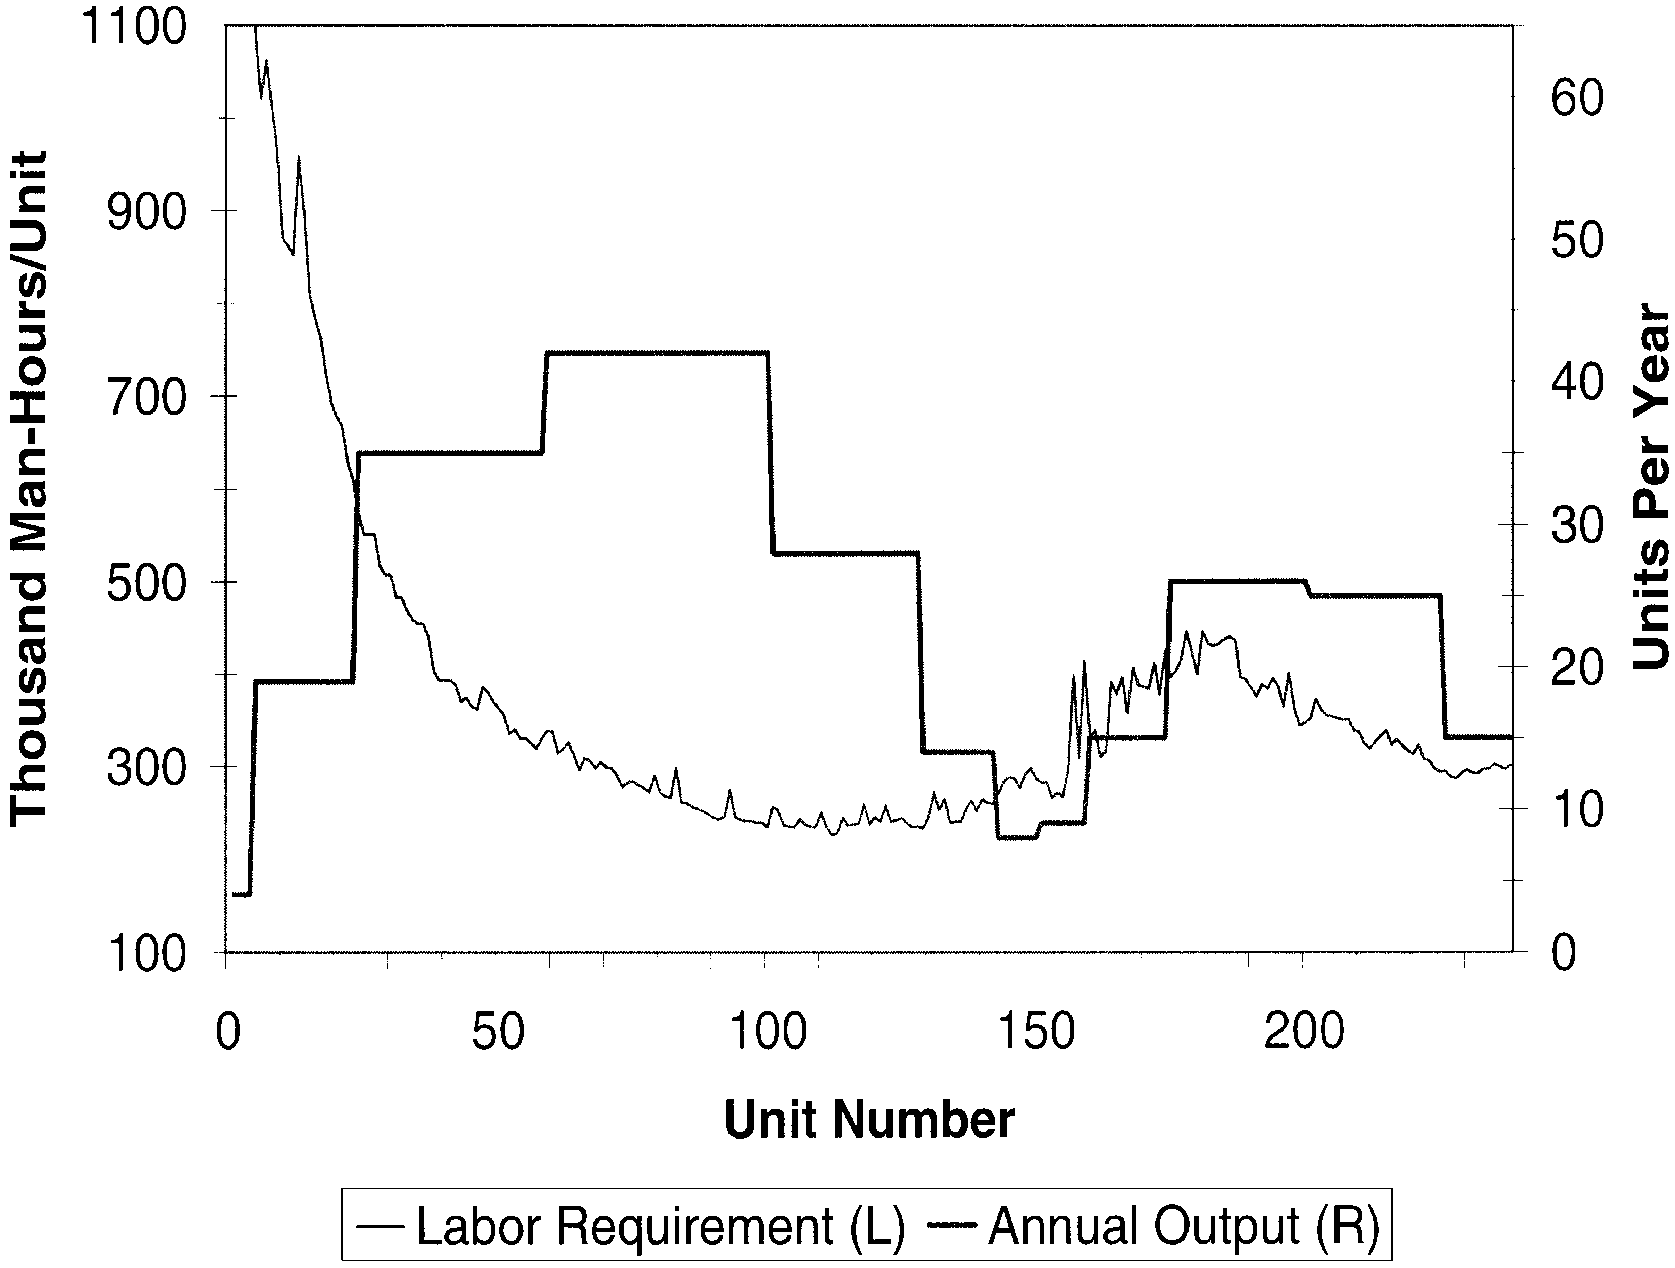
\includegraphics[height=5cm]{resources/learning_curve2.png}
		\caption{L-1011 Production: Direct Labor Requirement and Yearly Output. From: \citet[p. 1039]{Benkard2000}}
	\end{figure}
	\note{We see more than in the last picture. This is the production of the Lockheed L-1011. Famous for being an amazing plane, but a commercial failure. What happend here, around 150 units? Economic downturn, production was disrupted. Then, company decided the only way to break even is to produce a certain number of planes, but that did not happen.}
\end{frame}

\begin{frame}
	\frametitle{\insertsection}
	\framesubtitle{Disrupted learning}
	\begin{figure}
		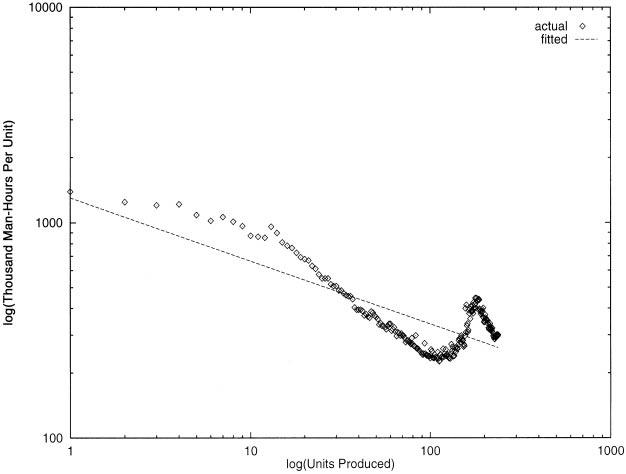
\includegraphics[height=5cm]{resources/learning_curve3.jpg}
		\caption{Traditional Learning Curve: All 238 (log-log). From: \citet[p. 1046]{Benkard2000}}
	\end{figure}
	\note{This is what actually happened. After Lockheed increased production again, the number of man-hours per plane actually increased for a while, before the price decreased again.}
\end{frame}

\begin{frame}
	Organizational forgetting
\end{frame}